\documentclass[11pt,reqno]{amsart}
\usepackage{amssymb,booktabs,tikz}
\usepackage[hidelinks]{hyperref}
\usepackage[capitalize,nameinlink,noabbrev]{cleveref}
\hypersetup{pdftitle={Optimality of a 25-Comparator Median Selection Network on Eleven Inputs},pdfauthor={Rocco Martino}}
\newcommand{\doi}[1]{\href{https://doi.org/#1}{doi:\nolinkurl{#1}}}
\newtheorem{theorem}{Theorem}[section]
\newtheorem{lemma}[theorem]{Lemma}
\newtheorem{proposition}[theorem]{Proposition}
\newtheorem{corollary}[theorem]{Corollary}
\newcommand{\wt}{\operatorname{wt}}
\title[Optimal median selection on eleven inputs]{Optimality of a 25-Comparator Median Selection Network on Eleven Inputs}
\author{Rocco Martino}
\date{24 November 2026, version 1.0.3}
\keywords{Comparator networks, order statistics, size optimality, computer-assisted proof}
\subjclass[2020]{68P10, 68Q17}
\begin{document}
\begin{abstract}
We prove that a fixed compare-exchange network needs at least 25
comparators to select the median of eleven inputs, even with arbitrary
depth, either gate orientation and a freely chosen fixed output wire.
Dobbelaere's 25-comparator construction attains the bound on the middle
wire. The lower bound follows from a deletion argument. Selecting one
rank fixes the entire output vector on each of two adjacent Boolean
weight layers. This forces an extreme input to traverse at least three
gates. A putative 24-gate network would therefore yield, after two
deletions, a network of at most 18 gates selecting rank four, five or
six on nine inputs. Rank duality and two certified finite exclusions
rule out all three cases. Lean~4 checks the exact-size theorem and the
decoded certificates for all 26 archived exclusions.
\end{abstract}
\maketitle

\section{Introduction}
A comparator network for a median filter can discard ordering information
as soon as the median is determined. An explicit circuit gives an upper
bound on its cost. A matching lower bound must exclude every shorter
sequence, including sequences of greater depth.
\begin{theorem}\label{thm:main}
Over any totally ordered domain containing at least two values, consider
eleven wires numbered $0,\ldots,10$. The minimum number of
compare-exchanges with the smaller output on the lower-numbered wire
that select the sixth smallest input on wire 5 is 25.
\end{theorem}
Dobbelaere's catalogue gives the construction used here \cite{dobb}.
Sekanina's eleven-input circuit has 26 compare-exchanges and 42 live
min/max subcomponents \cite[Table 3]{sekanina}. A later image-filter
study describes its seed circuits as optimal \cite{filter}. Neither
source supplies an exclusion of size 24 in our model. A report dated
16 November 2026 gives exact single-rank sizes through nine inputs,
including both base bounds used here \cite{gsi}. Our certificate rederives
the needed inequalities.

Yao studies networks selecting the smallest $t$ elements \cite{yao}.
Pippenger treats partition into two equally sized groups \cite{pippenger}.
Afshani et al.\ show that a single-rank network induces a fixed partition of
its outputs \cite[Lemmas 17--18]{afshani}. The two singleton images below
are a Boolean formulation of this phenomenon. Tomar proves a two-comparison
deletion step for selecting a group of largest elements \cite[Lemma 1.4]{tomar}
and uses extreme deletion for sorting \cite{tomarsort}. Smith published a
19-comparator median network for nine inputs, described it as minimal and
supplied no exclusion proof in the article \cite[Fig.~1]{smith}. Harder generalizes
the Van Voorhis deletion bound to sorting residual input sets and verifies
a certificate in Isabelle/HOL \cite{harder}. We specialize the path argument
to a single interior rank and combine it with a two-layer search. We found
no earlier proof of \cref{thm:main} in the sources examined.


\section{Model and threshold reduction}
An oriented gate $(a,b)$ has distinct ports. It writes the smaller of $x_a,x_b$
to $a$ and the larger to $b$. All other coordinates are unchanged.
A network is a fixed finite sequence of gates in the usual comparator model \cite{knuth}. Its size is its length.
It may use the same pair repeatedly. There is no fan-out, auxiliary storage,
constant source, adaptive branch, or restriction on depth. One fixed
coordinate is the output. For $1\le r\le n$ let $C(n,r)$ be the minimum
size with arbitrary orientations and free choice of that coordinate. Ranks
increase from one. The physical model in \cref{thm:main} requires $a<b$
and output 5. Its minimum is at least $C(11,6)$.

Let $H_s=\{x\in\{0,1\}^n:\wt(x)=s\}$ and $w=n-r$. Each gate preserves
weight and is monotone in the coordinatewise order, in either orientation.
For any threshold $t$ in a total order, applying $v\mapsto{\bf1}_{v\ge t}$
commutes with each gate and with the $r$th order statistic.
\begin{proposition}\label{prop:zero}
A fixed output selects rank $r$ on every input over a total order with at
least two values if and only if it is zero throughout $H_w$ and one
throughout $H_{w+1}$ in the Boolean model.
\end{proposition}
\begin{proof}
For necessity, use any strict pair in the domain as the two Boolean
values. For sufficiency, extend an input of weight at most $w$
up to weight $w$, or restrict one of weight at least $w+1$ to weight $w+1$.
Monotonicity gives the required bit. If an ordered output differs from the
desired value, the larger of the two values is a separating threshold.
This includes ties and requires no density assumption.
\end{proof}
The optimum is the same over any fixed domain with at least two ordered
values, since those values embed the Boolean test. Complementing the bits
and reversing every gate orientation interchanges $r$ and $n+1-r$.
Applying this operation twice gives $C(n,r)=C(n,n+1-r)$.

\begin{proposition}[Untangling, cf.\ {\cite[Section 2]{tomar}}]\label{prop:untangle}
$C(n,r)$ also equals the minimum for standard gates $a<b$ and prescribed
output $r-1$ in zero-based numbering.
\end{proposition}
\begin{proof}
Maintain a bijection from logical labels to physical wires, initially the
identity. For a logical gate compare the two labelled physical wires in
standard orientation. Assign the logical minimum port to the smaller
physical index and the other port to the larger. Induction gives the same
logical state at every step, with no physical swap gates. The final output
label maps to a fixed physical wire. On a strictly increasing input every
standard gate is idle, so the physical output must be wire $r-1$. Such
an input may be taken in the integers by \cref{prop:zero}. The reverse
inequality follows by inclusion.
\end{proof}
Thus the single-rank bounds in \cite{gsi} have the same output convention
after untangling. Our replay provides a self-contained basis for using them.

\section{Boundary-layer rigidity}
\begin{lemma}\label{lem:rigid}
If $F$ selects on wire $q$, there exists $u\in H_w$, $u_q=0$, such that
$F(H_w)=\{u\}$ and $F(H_{w+1})=\{u+e_q\}$.
\end{lemma}
\begin{proof}
For a cover $x\le y$ from $H_w$ to $H_{w+1}$, the outputs are comparable
and their weights differ by one. The selected coordinate changes from zero
to one, exhausting that difference. Thus $F(y)=F(x)+e_q$.
If $x,x'$ have weight $w$ and exchange one occupied position for another,
their union is a common upper neighbour. Subtracting $e_q$ gives
$F(x)=F(x')$. Given any two $w$-subsets, repeatedly move one element
outside the target into one missing position. The symmetric difference
decreases by two each time. This proves connectivity, including the
singleton case $w=0$. Every $(w+1)$-subset has a $w$-subset, also when
$w=n-1$. The cover identity gives the upper image.
\end{proof}
Conversely, if both images of a prefix are singletons, any cover exhibits
one differing coordinate, which separates the layers. On ordered distinct
keys the occupied positions on either side of the chosen rank can be read
by thresholding at that rank and just above it. This is the fixed-partition
property of \cite{afshani}.

\section{Deleting an extreme input}
\begin{lemma}\label{lem:three}
Suppose $\min(s,n-s)\ge4$ for some $s\in\{n-r,n-r+1\}$.
In every rank-$r$ network an original input position and a choice of
unique minimum or maximum exist whose route meets at least three gates.
\end{lemma}
\begin{proof}
The syntactic support of a wire starts as its input singleton. At a gate
both supports become the union of the two incoming supports. If all values
on a support are the same bit, the wire carries that bit, by induction.
A support of size at most four can be filled entirely with zeros or entirely
with ones while extending each assignment to the same $H_s$. Its wire varies
on that layer.

If all gates were disjoint, every final support would have size at most two,
contradicting \cref{lem:rigid}. Let $g$ be the earliest gate reusing a
wire and choose a reused port $a$. The preceding gates form a matching,
so exactly one earlier gate $h$ touched $a$. Put a unique minimum on an
input of $h$ if $a$ was its minimum output, a unique maximum otherwise.
It traverses $h$, stays at $a$ until $g$, and takes the corresponding output
of $g$. Each input of $g$ has support of size at most two. Even if both came
from $h$, the union has size at most four. The output carrying the extreme
therefore varies on $H_s$ and must be touched again by \cref{lem:rigid}.
At its next encounter the chosen extreme is still on that wire. The variation
test uses ordinary binary inputs to establish a property of the fixed wiring.
\end{proof}
\begin{lemma}[Deletion]\label{lem:delete}
Fix an input of an $m$-gate oriented network to a strict external sentinel.
If its route meets $d$ gates, the surviving output tuple, up to one fixed
bijection, is computed on $n-1$ wires with $m-d$ gates. If the original
network selects rank $r$, deleting a minimum selects $r-1$ when $r>1$,
and deleting a maximum selects $r$ when $r<n$.
\end{lemma}
\begin{proof}
Adjoin a value below, or above, the ordinary domain. Correctness extends
to it by \cref{prop:zero}. At time $t$ maintain the sentinel position $p_t$
and a bijection $\lambda_t$ from physical positions other than $p_t$ to
reduced wire labels. Initially use any enumeration of those positions.
The invariant is that each ordinary physical value equals the value at its
label for every assignment of the remaining inputs.

If $(a,b)$ misses $p_t$, append $(\lambda_t(a),\lambda_t(b))$ to the
reduced sequence and keep the bijection. Otherwise the sentinel takes its
prescribed output, $a$ for a minimum and $b$ for a maximum. Transfer the
label of the unique ordinary incoming port to the other outgoing port,
leaving all unaffected labels fixed. This is a bijection on the new
complement and requires no reduced gate. These updates prove the invariant
and count by induction. They depend only on the wiring and sentinel sign.
For the ranks specified, the selected value is ordinary. Hence the final
bijection maps the original output to a single fixed reduced wire.
Inserting the sentinel shifts the rank of each ordinary occurrence by one
for a minimum and zero for a maximum, also with repeated values.
\end{proof}
\begin{corollary}\label{cor:step}
For $1<r<n$ under the layer hypothesis of \cref{lem:three},
\[
 C(n,r)\ \ge\ 3+\min\{C(n-1,r-1),C(n-1,r)\}.
\]
\end{corollary}
\begin{proof}
Apply \cref{lem:three,lem:delete} to a minimum-size network. The witness
sign determines which reduced rank is available; the smaller cost bounds
both possibilities.
\end{proof}
The layer hypothesis matters. The median of three takes three comparators,
whereas adding three to either two-input extreme cost gives four.

\section{Finite lower bounds}\label{sec:finite}
A claim $(n,r,L)$ excludes every network of size at most $L$ in the enlarged
model. For a concrete prefix $P$ of length $p$ put
\[
 A=P(H_w),\qquad B=P(H_{w+1}),\qquad k=L-p.
\]
A \emph{completion} of $(A,B,k)$ is an oriented suffix of length at most
$k$ with a fixed output zero on all rows of $A$ and one on all rows of $B$.
By \cref{prop:zero} this is equivalent to completing $P$. The definition
refers to the two image sets alone.

\paragraph{Local exclusions.}
Every comparator has at most two preimages of any specified vector.
Outside the two ports the input is fixed, and inside them there are at
most two orders of the output pair. A layer with more than $2^k$ distinct
images cannot become a singleton in $k$ steps, as \cref{lem:rigid} requires.

For each original position and sign trace the route a strict sentinel would
take in $P$. Let $b$ be a previously proved lower bound for the rank after
deletion, or zero if none is available. On a valid rank deletion, a full
completion of total size at most $L$ must have at most $D=L-b$ encounters
on that path by \cref{lem:delete}. When deletion would remove the selected
rank itself, use only $D=L$, because each encounter uses one gate.
If a trace exceeds $D$, the prefix is impossible. If it attains $D$, its
present wire cannot be touched again. Variation of that wire \emph{within}
either layer therefore excludes the prefix. A difference solely between
layers does not suffice.

\paragraph{Enumeration.}
Try one representative $(i,j)$ with $i<j$ for each unordered pair.
The opposite orientation differs exactly by swapping the two output
labels. Conjugate every subsequent oriented gate and rename the terminal
coordinate by this transposition. This preserves existence and length of
a suffix. If the two discordant port patterns $10$ and $01$ do not both
occur in $A\cup B$, the gate acts there as one fixed permutation
(identity or transposition). Omitting it and conjugating the suffix gives
the same separation in one fewer step. The permutation need only agree on
these rows, since separation there implies correctness everywhere. Thus
a shortest nonempty completion can start with an enumerated pair. If the
representative violates a path cap, its exclusion rules out its reverse
as well, by conjugacy of completed networks.

\paragraph{Memoization.}
Permute both layers together, sorting wire labels stably by the pair of
column sums in $A,B$. Compare the two resulting \emph{entire} images.
Equal keys exhibit a specific common permutation. Ties can cause equivalent
states to have different keys, which only forgoes reuse. If a completed
exclusion with the same key allowed $k'\ge k$, conjugation transfers any
putative suffix to that earlier state. Even if the two prefixes have
different extreme traces, such a suffix appended to the \emph{earlier}
prefix would contradict its established exclusion at total budget
$|P_{\mathrm{earlier}}|+k'\le L$. A partial search of the earlier state
would not justify this inference.

\begin{proposition}[Replay soundness]\label{prop:replay}
Assume the smaller-width bounds used in replay. If replay accepts
$(n,r,L)$, then $C(n,r)>L$.
\end{proposition}
\begin{proof}
Associate to each closed node the proposition that its image pair has no
completion within its remaining budget. Check first that there is no
separating wire already, excluding the empty suffix. Cardinality and
frozen-wire leaves establish the proposition by the local exclusions.
A reference uses only a proposition already closed in the same claim.
For an expansion, choose a shortest hypothetical suffix. Its first gate
has a useful representative by the enumeration argument. A path violation
contradicts deletion; otherwise replay requires and checks the corresponding
child, whose proposition excludes the rest of the suffix. This proves the
parent proposition. Induct in order of node \emph{closure}, inserting an
expanded state only after its last child. The root has the original layers
and budget $L$. Induction over claims establishes all reported bounds:
the table is reset for each claim and cross-claim dependencies have
strictly smaller width.
\end{proof}

\begin{center}
\begin{minipage}{0.96\linewidth}\small
\textbf{Replay of an implicit preorder tree}\\[2pt]
\texttt{visit}$(P,A,B,k)$: consume one opcode; reject a current separator.\\
\hspace*{1em}1: verify $\max(|A|,|B|)>2^k$; return.\\
\hspace*{1em}2: find a closed common-permutation key with budget $\ge k$; return.\\
\hspace*{1em}3: find a saturated trace on a within-layer varying wire; return.\\
\hspace*{1em}0: require $k>0$; enumerate $i<j$ in lexicographic order.\\
\hspace*{2em}Skip fixed permutations and pairs exceeding a trace allowance.\\
\hspace*{2em}For each remaining $g$, call \texttt{visit}$(Pg,gA,gB,k-1)$.\\
\hspace*{2em}Record the closed key and budget.\\
Reject failed predicates, invalid opcodes, missing bytes and trailing nodes.
\end{minipage}
\end{center}

\section{The exact size}
\begin{proof}[Proof of \cref{thm:main}]
Apply \cref{prop:replay} to $(9,4,18)$ and $(9,5,18)$. Both nine-input
ranks require at least 19 comparators. Duality gives $C(9,6)\ge19$.
The layer of weight five has respectively five and six zeros at widths ten
and eleven. It is a boundary layer for each of $(10,5),(10,6),(11,6)$.
Applying \cref{cor:step} to the first two gives a lower bound of 22 in
both cases. Applying it to the third gives 25. This suffices for the
fixed-wire, lower-index-minimum model. For the opposite inequality, the
25 comparators in \cref{fig:net} yield the required bit on wire 5 on all
$2^{11}$ binary inputs by exhaustive evaluation. Apply \cref{prop:zero}.
\end{proof}

\section{Verification and reproducibility}
The certificate consists of a JSON list of triples and one gzip member per
triple. The uncompressed bytes are the opcodes above. Lexicographic child
order supplies the implicit tree boundaries; reference targets are looked
up by image key and budget. The generator uses integer bitsets and forward
maximum path lengths. The Python checker uses sets and tracks each possible
extreme separately. The C++ checker stores a sorted union of distinct words;
weight recovers the layer. At each expanded or frozen node it scans the
gate list \emph{backwards}. Initially each port has destiny $(i,0)$. At a
reversed gate, for a given sign, let $(j,d)$ be the destiny of the extreme
output. Both input ports receive $(j,d+1)$. Backward induction gives the
terminal wire and encounter count for each starting position. No generator
code or stored node counts enter this calculation.

\begin{table}[ht]
\centering\small
\caption{Completed replays. Lower bounds are in order of ascending rank;
node counts are summed within each width.}
\label{tab:counts}
\begin{tabular}{rllr}\toprule
$n$&Ranks&Lower bounds&Nodes\\\midrule
2&1&1&1\\
3&1--2&2, 3&5\\
4&1--2&3, 5&8\\
5&1--3&4, 7, 7&23\\
6&1--3&5, 9, 10&106\\
7&1--4&6, 11, 12, 13&124\\
8&1--4&7, 13, 14, 16&5\,006\\
9&1--5&8, 15, 16, 19, 19&168\,163\\
10&5&22&256\\
11&6&25&316\\\midrule
\multicolumn{3}{l}{Total for 26 claims}&174\,008\\\bottomrule
\end{tabular}
\end{table}

Both replays returned the counts in \cref{tab:counts}. The $(9,4)$ claim
alone takes 167\,917 nodes, $(9,5)$ takes 171. The regenerated manifest,
all 26 compressed files and the generator's diagnostic log matched the
distributed copies byte for byte in the audit environment. The two
large-width claims give direct replays in addition to the analytic
recurrence, sharing smaller-width dependencies.

An independent exhaustive search for $n\le6$ represents one output by
its entire Boolean truth table. At distance zero take all projections.
From $f$, visit $f\circ g$ for every ordered gate $g$. Induction on distance
identifies the frontier with the functions first reachable at that size:
prepending a gate composes the output in precisely this way. First discovery
of a rank threshold gives its minimum. This calculation uses no boundary
restriction, path pruning, wire symmetry or certificate. It returned the
costs in \cref{tab:counts} and their duals for all 20 ranks at widths two
through six. A separate simulation checked all $3^{11}=177\,147$ ternary
inputs. Deleting each single gate in turn produced 25 circuits with between
21 and 490 failing binary inputs apiece.

\paragraph{Artifact.}
The full replays can be run from the repository root:
\begin{verbatim}
python3 verify.py median11_25.json
python3 -O check_certificate.py
g++ -std=c++20 -O2 verification/independent/check.cpp \
    -lz -o check
./check certificate
\end{verbatim}
The \href{https://github.com/HaxelThePenguine/median-of-11}{project repository}
includes the proof bytes, implementation and audit record;
see \texttt{docs/reproducibility.md} and \texttt{docs/certificate.md}.

\section{Scope and limitations}
The computed objects are lower bounds. The upper bound at eleven has its
own explicit witness. The argument does not determine optimal depth
at size 25, adaptive comparison cost, or the cost of circuits that charge
separately for minimum and maximum. Codish et al.\ use hybrid search and
SAT for sorting \cite{codish}. Our certificate checks combinatorial
exclusions directly. The historical SAT runs for the unrestricted
size-24 instance returned unknown. No SAT unsatisfiability proof or LRAT
checker \cite{lrat} enters the result.

The two checkers share a mathematical specification and a proof stream.
Their agreement detects implementation errors but cannot rule out a common
mistake in the specification. A Lean 4 development proves the cover and
constancy implications from fixed-width weight conservation, monotonicity
of the remaining coordinates and boundary separation. The extreme-path
argument and certificate replay are justified by the mathematical proofs
above. Their implementations have not been verified in a proof assistant.
The repository and this audit were developed with AI assistance; independent
implementation here describes software independence within the project.

\appendix
\section{The upper-bound witness}
\begin{figure}[ht]
\centering
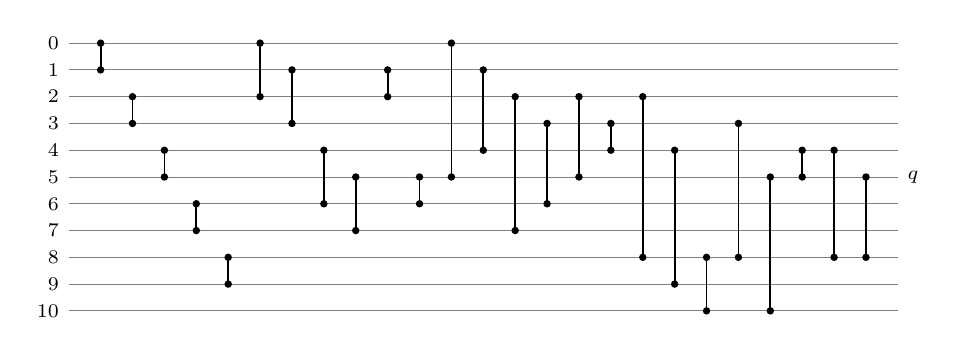
\begin{tikzpicture}[x=.405cm,y=-.34cm]
\foreach \i in {0,...,10} {
  \draw[black!50,line width=.35pt] (0,\i)--(26,\i);
  \node[left,font=\scriptsize] at (0,\i) {\i};
}
\newcommand{\gate}[3]{
  \draw[line width=.65pt] (#1,#2)--(#1,#3);
  \fill (#1,#2) circle[radius=1.35pt] (#1,#3) circle[radius=1.35pt];
}
\gate{1}{0}{1}
\gate{2}{2}{3}
\gate{3}{4}{5}
\gate{4}{6}{7}
\gate{5}{8}{9}
\gate{6}{0}{2}
\gate{7}{1}{3}
\gate{8}{4}{6}
\gate{9}{5}{7}
\gate{10}{1}{2}
\gate{11}{5}{6}
\gate{12}{0}{5}
\gate{13}{1}{4}
\gate{14}{2}{7}
\gate{15}{3}{6}
\gate{16}{2}{5}
\gate{17}{3}{4}
\gate{18}{2}{8}
\gate{19}{4}{9}
\gate{20}{8}{10}
\gate{21}{3}{8}
\gate{22}{5}{10}
\gate{23}{4}{5}
\gate{24}{4}{8}
\gate{25}{5}{8}

\node[right,font=\scriptsize] at (26,5) {$q$};
\end{tikzpicture}
\caption{Dobbelaere's 25-comparator network \cite{dobb}, serialized in
execution order. Dots identify the two participating ports. The smaller
value leaves the upper dot.}
\label{fig:net}
\end{figure}
Writing $ab$ for $(a,b)$ with $t=10$, the disjoint gates at each successive
level are
\[
\begin{gathered}
01,\ 23,\ 45,\ 67,\ 89 \quad|\quad 02,\ 13,\ 46,\ 57
 \quad|\quad 12,\ 56\\
05,\ 14,\ 27,\ 36 \quad|\quad 25,\ 34 \quad|\quad 28,\ 49
 \quad|\quad 8t\\
38,\ 5t \quad|\quad 45 \quad|\quad 48 \quad|\quad 58 .
\end{gathered}
\]
The verifier evaluates these gates as given in \texttt{median11\_25.json}
for masks 0 through 2047, with bit $i$ on wire $i$. The expected output is
$\mathbf{1}_{\wt(x)\ge6}$.

\bibliographystyle{plain}
\bibliography{references}
\end{document}
